\chapter{A Shifting Reef}

The year 1866 was signalised by a remarkable incident, a mysterious
and puzzling phenomenon, which doubtless no one has yet forgotten.
Not to mention rumours which agitated the maritime population
and excited the public mind, even in the interior of continents,
seafaring men were particularly excited.  Merchants, common sailors,
captains of vessels, skippers, both of Europe and America,
naval officers\cite{article-full} of all countries, and the 
Governments of several States
on the two continents, were deeply interested in the matter.

For some time past vessels had been met by ``an enormous thing,''
a long object, spindle-shaped, occasionally phosphorescent,
and infinitely larger and more rapid in its movements than a whale.

\section{Add a section marker here}

The facts relating to this apparition (entered in various log-books)
agreed in most respects as to the shape of the object or creature in question,
the untiring rapidity of its movements, its surprising power of locomotion,
and the peculiar life with which it seemed endowed.  If it was a whale,
it surpassed in size all those hitherto classified in science.
Taking into consideration the mean of observations made at divers 
times---rejecting the timid estimate of those who assigned to this object
a length of two hundred feet, equally with the exaggerated opinions
which set it down as a mile in width and three in length---we might fairly
conclude that this mysterious being surpassed greatly all dimensions
admitted by the learned ones of the day, if it existed at all.
And that it DID exist was an undeniable fact; and, with that tendency
which disposes the human mind in favour of the marvellous, we can understand
the excitement produced in the entire world by this supernatural apparition.
As to classing it in the list of fables, the idea was out of the question.

\section{Add another section marker}

\begin{equation}
E=mc^2
\end{equation}

On the 20th of July, 1866, the steamer Governor Higginson,
of the Calcutta and Burnach Steam Navigation Company, had met
this moving mass five miles off the east coast of Australia.
Captain Baker thought at first that he was in the presence of an
unknown sandbank; he even prepared to determine its exact position
when two columns of water, projected by the mysterious object,
shot with a hissing noise a hundred and fifty feet up into the air.
Now, unless the sandbank had been submitted to the intermittent
eruption of a geyser, the Governor Higginson had to do neither
more nor less than with an aquatic mammal, unknown till then,
which threw up from its blow-holes columns of water mixed with
air and vapour.\cite{inbook-full}\cite{book-full}

Similar facts were observed on the 23rd of July in the same year,
in the Pacific Ocean, by the Columbus, of the West India
and Pacific Steam Navigation Company.  But this extraordinary
creature could transport itself from one place to another
with surprising velocity; as, in an interval of three days,
the Governor Higginson and the Columbus had observed it at
two different points of the chart, separated by a distance
of more than seven hundred nautical leagues.

\section{extra section marker}

Fifteen days later, two thousand miles farther off, the Helvetia,
of the Compagnie-Nationale, and the Shannon, of the Royal
Mail Steamship Company, sailing to windward in that portion
of the Atlantic lying between the United States and Europe,
respectively signalled the monster to each other in 42@ 15' N. lat.
and 60@ 35' W. long.  In these simultaneous observations they
thought themselves justified in estimating the minimum length
of the mammal at more than three hundred and fifty feet,
as the Shannon and Helvetia were of smaller dimensions than it,
though they measured three hundred feet over all.

Now the largest whales, those which frequent those parts of the sea round
the Aleutian, Kulammak, and Umgullich islands, have never exceeded the length
of sixty yards, if they attain that.

\begin{equation}
E=mc^2
\end{equation}

In every place of great resort the monster was the fashion.
They sang of it in the cafes, ridiculed it in the papers, and represented
it on the stage.  All kinds of stories were circulated regarding it.
There appeared in the papers caricatures of every gigantic and
imaginary creature, from the white whale, the terrible ``Moby Dick''
of sub-arctic regions, to the immense kraken, whose tentacles could entangle
a ship of five hundred tons and hurry it into the abyss of the ocean.
The legends of ancient times were even revived.

Then burst forth the unending argument between the believers and the
unbelievers in the societies of the wise and the scientific journals.
``The question of the monster'' inflamed all minds.  Editors of
scientific journals, quarrelling with believers in the supernatural,
spilled seas of ink during this memorable campaign, some even drawing blood;
for from the sea-serpent they came to direct personalities.

\section{another section marker}

During the first months of the year 1867 the question seemed buried,
never to revive, when new facts were brought before the public.
It was then no longer a scientific problem to be solved, but a real
danger seriously to be avoided.  The question took quite another shape.
The monster became a small island, a rock, a reef, but a reef of indefinite
and shifting proportions.

\subsection{a subsection marker}

On the 5th of March, 1867, the Moravian, of the Montreal Ocean Company,
finding herself during the night in 27@ 30' lat.  and 72@ 15' long., struck
on her starboard quarter a rock, marked in no chart for that part of the sea.
Under the combined efforts of the wind and its four hundred horse power,
it was going at the rate of thirteen knots.  Had it not been for the superior
strength of the hull of the Moravian, she would have been broken by the shock
and gone down with the 237 passengers she was bringing home from Canada.

The accident happened about five o'clock in the morning, as the day
was breaking.  The officers of the quarter-deck hurried to the after-part
of the vessel.  They examined the sea with the most careful attention.
They saw nothing but a strong eddy about three cables' length distant,
as if the surface had been violently agitated.  The bearings of the place were
taken exactly, and the Moravian continued its route without apparent damage.
Had it struck on a submerged rock, or on an enormous wreck?  They could
not tell; but, on examination of the ship's bottom when undergoing repairs,
it was found that part of her keel was broken.

\subsection{another subsection}

This fact, so grave in itself, might perhaps have been forgotten
like many others if, three weeks after, it had not been re-enacted
under similar circumstances.  But, thanks to the nationality of
the victim of the shock, thanks to the reputation of the company to
which the vessel belonged, the circumstance became extensively circulated.

The 13th of April, 1867, the sea being beautiful, the breeze favourable,
the Scotia, of the Cunard Company's line, found herself in 15@ 12' long.
and 45@ 37' lat.  She was going at the speed of thirteen knots and a half.

At seventeen minutes past four in the afternoon, whilst the passengers were
assembled at lunch in the great saloon, a slight shock was felt on the hull
of the Scotia, on her quarter, a little aft of the port-paddle.

\begin{figure}%
  \centering
  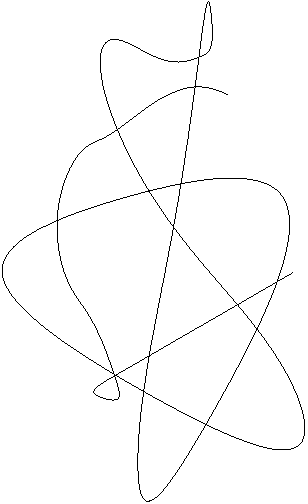
\includegraphics[width=100bp]{jules-verne-test}%
  \caption[A test figure. This is a test figure inserted into this text.  This is a test figure inserted into this text.  This is a test figure inserted into this text.]
  {This is a test figure inserted into this text.}%
  \label{fig:test1}%
\end{figure}

The Scotia had not struck, but she had been struck, and seemingly
by something rather sharp and penetrating than blunt.
The shock had been so slight that no one had been alarmed,
had it not been for the shouts of the carpenter's watch,
who rushed on to the bridge, exclaiming, ``We are sinking! we
are sinking!''  At first the passengers were much frightened,
but Captain Anderson hastened to reassure them.  The danger could
not be imminent.  The Scotia, divided into seven compartments
by strong partitions, could brave with impunity any leak.
Captain Anderson went down immediately into the hold.
He found that the sea was pouring into the fifth compartment;
and the rapidity of the influx proved that the force of the water
was considerable.  Fortunately this compartment did not hold
the boilers, or the fires would have been immediately extinguished.
Captain Anderson ordered the engines to be stopped at once,
and one of the men went down to ascertain the extent of the injury.
Some minutes afterwards they discovered the existence of a
large hole, two yards in diameter, in the ship's bottom.
Such a leak could not be stopped; and the Scotia, her paddles
half submerged, was obliged to continue her course.  She was then
three hundred miles from Cape Clear, and, after three days' delay,
which caused great uneasiness in Liverpool, she entered the basin
of the company.

\subsubsection{a subsubsection with a really really really really really really really really really really long title. I mean a really really really really really really really really really really long title. No, even longer than that.}

The engineers visited the Scotia, which was put in dry dock.
They could scarcely believe it possible; at two yards and a half below
water-mark was a regular rent, in the form of an isosceles triangle.
The broken place in the iron plates was so perfectly defined
that it could not have been more neatly done by a punch.
It was clear, then, that the instrument producing the perforation
was not of a common stamp and, after having been driven with
prodigious strength, and piercing an iron plate 1 3/8 inches thick,
had withdrawn itself by a backward motion.

\subsubsection{a subsubsection with shorter title}

Such was the last fact, which resulted in exciting once more the torrent
of public opinion.  From this moment all unlucky casualties which could
not be otherwise accounted for were put down to the monster.

\section{a final section}

Upon this imaginary creature rested the responsibility of all
these shipwrecks, which unfortunately were considerable;
for of three thousand ships whose loss was annually recorded
at Lloyd's, the number of sailing and steam-ships supposed
to be totally lost, from the absence of all news, amounted to
not less than two hundred!

Now, it was the ``monster'' who, justly or unjustly, was accused
of their disappearance, and, thanks to it, communication between
the different continents became more and more dangerous.
The public demanded sharply that the seas should at any price be
relieved from this formidable cetacean.\footnote{Member of the whale family.}

